\documentclass{article}

% if you need to pass options to natbib, use, e.g.:
%     \PassOptionsToPackage{numbers, compress}{natbib}
% before loading neurips_2021

% ready for submission
\usepackage[preprint]{neurips_2023}

% to compile a preprint version, e.g., for submission to arXiv, add add the
% [preprint] option:
%     \usepackage[preprint]{neurips_2021}

% to compile a camera-ready version, add the [final] option, e.g.:
%     \usepackage[final]{neurips_2021}

% to avoid loading the natbib package, add option nonatbib:
%    \usepackage[nonatbib]{neurips_2021}

\usepackage[utf8]{inputenc} % allow utf-8 input
\usepackage[T1]{fontenc}    % use 8-bit T1 fonts
\usepackage[colorlinks=true]{hyperref}       % hyperlinks
\usepackage{url}            % simple URL typesetting
\usepackage{booktabs}       % professional-quality tables
\usepackage{amsfonts}       % blackboard math symbols
\usepackage{nicefrac}       % compact symbols for 1/2, etc.
\usepackage{microtype}      % microtypography
\usepackage{xcolor}         % colors
\usepackage{graphicx}

\title{Corporate vs. Academia: Who Dominates CV Conferences?}

% The \author macro works with any number of authors. There are two commands
% used to separate the names and addresses of multiple authors: \And and \AND.
%
% Using \And between authors leaves it to LaTeX to determine where to break the
% lines. Using \AND forces a line break at that point. So, if LaTeX puts 3 of 4
% authors names on the first line, and the last on the second line, try using
% \AND instead of \And before the third author name.

\author{%
  Irem Karaca\\
  Matrikelnummer 6939373\\
  \texttt{@student.uni-tuebingen.de} \\
  \And
  Merve Kocabas\\
  Matrikelnummer 7040890\\
  \texttt{merve.kocabas@student.uni-tuebingen.de} \\
  \And
  Hari Joshithaa Aghilah Senthilprathiban\\
  Matrikelnummer 6943473\\
  \texttt{hari-joshitha.aghilah-senthilprathiban@student.uni-tuebingen.de} \\
  \And
  Shubham Raheja\\
  Matrikelnummer 7001572\\
  \texttt{@student.uni-tuebingen.de} \\
}

\begin{document}

\maketitle

\begin{abstract}
  % \emph{[Use this abstract to briefly explain what you are planning to do. Here is an example:]} We are planning to use the collection of \href{https://openreview-py.readthedocs.io/en/latest/getting_data.html}{all papers ever \emph{submitted} to the ICLR conference} to see how well paper acceptance can be predicted from trivial features, such as the paper's overall length, number of words or number of figures. We are planning to use logistic regression for this purpose.

  In this project, we analyse the corporate and academia involvement in popular Computer Vision conferences such as CVPR, ICCV and WACV. 
\end{abstract}

% You can find a detailed example and instructions on how to use this style file in the attached \texttt{neurips\_2023.tex} file. This includes instructions for how to lay out citations.

\section{Introduction}


\section{Data and Methods}



\section{Results}
To explore the hypothesis—Do papers from corporate-affiliated researchers have more influence at top-tier computer vision conferences?—we begin by examining the trend in the quantity of corporate-affiliated papers over the years. As shown in Figure \ref{fig:corporate_ratio_graph}, the proportion of corporate-affiliated papers has steadily increased across major computer vision conferences. CVPR, ICCV, WACV, and the combined dataset all exhibit a consistent upward trend, with corporate involvement reaching its highest levels in recent years. However, despite this increase, academia continues to dominate these conferences, as the highest ratio of corporate-affiliated papers remains at 0.47. Additionally, while ICCV and CVPR show relatively higher levels of corporate affiliation, WACV consistently lags behind them in this regard. The Spearman rank correlation results in Table \ref{tab:spearman_results} further support the observation in consistent upward trend in corporate affiliation, with strong positive correlations (coefficients exceeding 0.88) and statistically significant p-values (all below 0.05). These findings illustrate the growing presence of corporate-affiliated research within the academic ecosystem of top-tier computer vision venues.

\begin{figure}[ht]
  \centering
  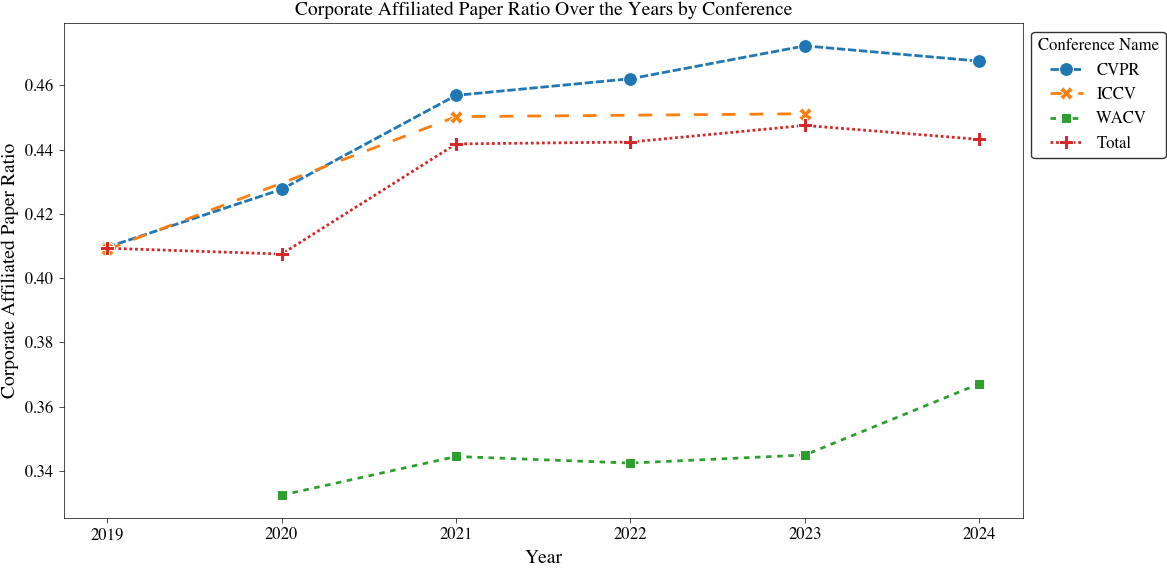
\includegraphics[width=\textwidth]{../images/corporate_ratio_graph_final.png}  
  \caption{Corporate affiliated paper ratio over the years for each conference and total dataset.}
  \label{fig:corporate_ratio_graph}
\end{figure}

\begin{table}[ht]
\centering
\begin{tabular}{|l|c|c|c|}
\hline
\textbf{Conference} & \textbf{Spearman Rank Correlation} & \textbf{P-value} & \textbf{Significant Relationship?} \\ \hline
CVPR & 0.9429 & 0.0048 & Yes \\ \hline
ICCV & 1.0000 & 0.0000 & Yes \\ \hline
WACV & 0.9000 & 0.0374 & Yes \\ \hline
Total & 0.8857 & 0.0188 & Yes \\ \hline
\end{tabular}
\caption{Spearman rank correlation results for each conference and total dataset.}
\label{tab:spearman_results}
\end{table}

Building on the observed upward trend in corporate-affiliated papers, we now turn our attention to their impact. A critical metric for evaluating research influence is citation count, which reflects the reach and recognition of a paper within the scientific community. To assess this, we compare the citation performance of corporate-affiliated papers to those from academia across top-tier computer vision conferences. Specifically, we examine whether corporate-affiliated papers, despite their lower overall proportion, exhibit higher citation counts, thereby offering insight into their relative impact as hypothesized.


\section{Discussion and Conclusion}

\section{Future Work}

\section{Contributions Statement}
% This is the last section before the references. 

% \emph{Here is an example:}

% XX performed the correlation analysis, organized the data and code for the processing of dataset1 and subdataset2, and created the scatter plot. 
% YY created the random forest regression model, performed the data cleaning for the xyz analysis / xyz database, and created the bar charts to display the regression results. 
% ZZ researched and collected the raw data, restructured the pipeline for the data analysis, and proof-read the draft for the final report. 
% AA performed the data cleaning for dataset1, and performed the Ridge and Lasso regularization. 
% All members of the group contributed to writing the report.

\section*{References}

\end{document}
